\documentclass{article}
\usepackage[utf8]{inputenc}
\usepackage{geometry}
\usepackage{graphicx}
\usepackage{pgfplots}
\usepackage{verbatim}
\usepackage{amssymb}
\usepackage{amsmath}
\usepackage{tcolorbox} %needed
\usepackage{comment}
\tcbuselibrary{listingsutf8}
\newcommand{\abs}{\biggm|}
\newcommand{\ints}{\displaystyle \int \!}
\newcommand{\phix}{\varphi (x)}
\newcommand{\gammax}{\gamma (x)}
\newcommand{\psix}{\psi (x)}
\newcommand{\mux}{\mu (x)}
\newcommand{\thetax}{\vartheta (x)}
\newcommand{\xix}{\xi (x)}
\newcommand{\etax}{\eta (x)}
\newcommand{\upx}{\upsilon (x)}
\newcommand{\qed}{\quad\quad\quad\mathfrak{QED}}
\newcommand{\arcsinh}{\text{arcsinh}}
\newcommand{\A}{\mathfrak{A}}
\newcommand{\B}{\mathfrak{B}}
\newcommand{\plic}{\quad \implies \quad}

\geometry{a4paper, left=2cm, right=2cm, top=1cm, bottom=2cm}
\pgfplotsset{compat=1.18}

\begin{document}

% Problema XII
\noindent XII. $\ints \sqrt{e^x + 1} \, dx$\\
\begin{center}
\begin{tcolorbox}[title=Considérese el siguiente cambio de variable, width=0.7\linewidth]
    \(
    \phix = \sqrt{1 + e^x} \plic d\phix = \frac{e^x}{2\sqrt{1 + e^x}}dx \quad \implies dx = \frac{2\phix d\phix}{\phix^2 -1} \\
    \phix^2 = 1 + e^x \plic \phix^2 - 1 = e^x
    \)
\end{tcolorbox}
\end{center}
\(
\ints \sqrt{e^x + 1} \, dx = \ints \frac{2\phix^2 d\phix}{\phix^2 - 1} = \ints \frac{2\phix^2 + [2-2]}{\phix^2 - 1} \, d\phix = \ints 2 \left[\frac{\phix^2-1}{\phix^2-1}\right] \, d\phix + 2 \ints\frac{d\phix}{\phix^2 -1} \\\\\\
2\phix + 2 \ints\frac{d\phix}{\phix^2 -1} = 2\phix + 2^{-1}ln\left[\frac{\phix + 1}{\phix - 1}\right] + c = 2\sqrt{1+e^x} + ln\left[\frac{\sqrt{1+e^x} - 1}{\sqrt{1+e^x} + 1}\right] + c \qed
\)
\\\\\\\\

% Problema XIII
\noindent XIII. $\ints \dfrac{5x^2 + 6x + 9}{(x-3)^2(x+1)^2} \, dx$
\begin{center}
\begin{tcolorbox}[title=Método de reducción por fracciones parciales, width=0.7\linewidth, top=0pt]
\begin{align*}
    \frac{5x^2 + 6x + 9}{(x-3)^2(x+1)^2} &= \frac{\A}{(x-3)^2} + \frac{\B}{(x+1)} \\
    5x^2 + 6x + 9 &= (x+1)^2\A + (x-3)^2\B \\
    \textit{\textbf{Sea x igual a -1}}& \\
    5 - 6 + 9 = 8 &= 0\A + (-4)^2 \B = 16 \B \plic \B = \frac{8}{16} = 2^{-1} \\
    \textit{\textbf{Sea x igual a 3}}& \\
    45 + 18 + 9 = 72 &= 16 \A \plic \A = \frac{72}{16}= \frac{9}{2}
\end{align*}
\end{tcolorbox}
\end{center}
\(
\ints \dfrac{5x^2 + 6x + 9}{(x-3)^2(x+1)^2} \, dx = \ints \frac{\A}{(x-3)^2} + \frac{\B}{(x+1)} \, dx = \frac{9}{2}\ints \frac{dx}{(x-3)^2} + 2^{-1}\ints \frac{dx}{(x+1)^2}
\)
\begin{center}
\begin{tcolorbox}[title=Considérense los siguientes cambios de variable, width=0.7\linewidth, top=0pt]
\begin{align*}
    \phix = x-3 &\quad \gammax = x+1 \\
    d\phix = dx &\quad \gammax = dx
\end{align*}
\end{tcolorbox}
\end{center}
\(
\dfrac{9}{2}\ints \frac{dx}{(x-3)^2} + 2^{-1}\ints \frac{dx}{(x+1)^2} = \frac{9}{2} \ints \frac{d\phix}{\phix^2} + \frac{1}{2} \ints \frac{d\gammax}{\gammax^2} = \frac{9\phix^{-1}}{-2} + \frac{\gammax^{-1}}{-2} + c = \frac{9}{-2\phix} + \frac{1}{-2\gammax} \\\\\\
= - \frac{9}{2x-6} -  \frac{1}{2x+2} + c \qed
\)
\\\\\\\\

% Problema XIV
\noindent XIV.  $\ints \frac{3x+5}{(x^2+2x+2)^2} \, dx$ \\\\\\
\(
\ints \frac{3x+5}{(x^2+2x+2)^2} \, dx = \ints \frac{[3x+3] + [2]}{(x^2+2x+2)^2} \, dx = \ints \frac{3x+3}{(x^2+2x+2)^2} \, dx + \ints \frac{2}{(x^2+2x+2)^2} \, dx
\)
\begin{center}
\begin{tcolorbox}[title=Considérense los siguientes cambios de variable, width=0.7\linewidth, top=0pt]
\begin{align*}
    \phix = x^2+2x+2 \quad \mux &= x + 1 \quad \thetax = \arctan[\mux] \\
    d\phix = (2x+2)dx \quad d\mux &= dx \quad\quad d\thetax = [(\mux)^2+1^2]^{-1}dx \\
    &\hspace{1.5cm} tan[\thetax] = \mux = x+1
\end{align*}
\end{tcolorbox}
\end{center}
\(
\ints \frac{3x+3}{(x^2+2x+2)^2} \, dx + \ints \frac{2}{(x^2+2x+2)^2} \, dx = \frac{3}{2} \ints \frac{d\phix}{\phix^2} + 2 \ints \frac{dx}{[(x+1)^2+1]^2} = \frac{3}{2} \ints \frac{d\phix}{\phix^2} + 2 \ints \frac{d\mux}{[\mux^2+1]^2} \\\\\\
= \frac{3}{2} \ints \frac{d\phix}{\phix^2} + 2 \ints \frac{d\thetax}{\sec^4[\thetax]\cos^2[\thetax]} = \frac{3}{2} \ints \frac{d\phix}{\phix^2} + 2\ints \frac{\cos^4[\thetax]d\thetax}{\cos^2[\thetax]} = -\frac{3}{2\phix} + 2\ints \cos^2[\thetax]d\thetax \\\\\\
= -\frac{3}{2\phix} + 2\ints \frac{1 + \cos[2\thetax]}{2}d\thetax = -\frac{3}{2\phix} + 2\left[2^{-1}\thetax + 4^{-1}\sin[2\thetax]\right] = -\frac{3}{2\phix} + \thetax + 2^{-1}\sin[2\thetax] \\\\\\
= -\frac{3}{2\phix} + \arctan[\mux] + \frac{\sin[2\arctan[\mux]]}{2} = -\frac{3}{2x^2+4x+4} + \arctan(x+1) + \frac{\sin[2\arctan(x+1)]}{2} + c \quad\quad\mathfrak{QED}
\)
\\\\\\\\

% Problema XV
\noindent XV.  $\ints \frac{\sqrt{x+1} + 2}{(x+1)^2 - \sqrt{x+1}}dx$ \\
\begin{center}
\begin{tcolorbox}[title=Considérese en un futuro el siguiente cambio de variable, width=0.7\linewidth, top=0pt]
    \[
    \phix = \sqrt{x+1} \plic d\phix = \frac{dx}{2\sqrt{x+1}}
    \]
    \textit{Asímismo recuérdese lo siguiente...   }
    $(\alpha^2-\alpha)(\alpha^2+\alpha+1) = \alpha^4 - \alpha$
\end{tcolorbox}
\end{center}
\(
\ints \frac{\sqrt{x+1} + 2}{(x+1)^2 - \sqrt{x+1}}dx = \ints \frac{[\sqrt{x+1} + 2]dx}{((x+1)-\sqrt{x+1})((x+1)+\sqrt{x+1}+1)} = \ints \frac{[-\sqrt{x+1} - 2]dx}{(\sqrt{x+1}+(x+1))((x+1)+\sqrt{x+1}+1)} \\\\\\
= \ints 2^{-1} \frac{[-2\sqrt{x+1} - 4]dx}{(\sqrt{x+1}+(x+1))((x+1)+\sqrt{x+1}+1)} = \ints \left[\frac{dx}{2\sqrt{x+1}}\right] \left[\frac{-2\sqrt{x+1} - 4}{(1-\sqrt{x+1})([x+1]+\sqrt{x+1}+1)}\right] \\\\\\
= \ints \frac{-2u - 4}{(1-u)(u^2+u+1)} \, du = \ints \frac{(2u^2-2)-2u^2-2u-2}{(1-u)(u^2+u+1)} \, du = \ints \frac{(-2u-2)(1-u)-(2u^2+2u+2)}{(1-u)(u^2+u+1)} \\\\\\
=\ints \frac{-2u-2}{u^2+u+1} - \frac{2}{1-u} \, du = \ints -\frac{2u+1}{u^2+u+1} -\frac{1}{u^2+u+1} - \frac{2}{1-u} \, du = \ints -\frac{1}{u^2+u+1} - \frac{2}{1-u} -\frac{2u+1}{u^2+u+1} \\\\\\
= \left[- \ints \frac{du}{u^2+u+1} \right] + 2\ln|u-1| - \ln|u^2+u+1| \hspace{2.78cm}\dotfill \textit{nos enfocaremos en la integral restante}\\\\\\
- \ints \frac{du}{u^2+u+1} = - \ints \frac{4du}{4u^2+4u+4} = -4 \ints \frac{du}{[2u+1]^2+3} = \ints -\frac{4}{3} \cdot \frac{du}{[\frac{2u+1}{\sqrt{3}}]^2+1} = \ints -\frac{2}{\sqrt{3}} \cdot \frac{du}{[\frac{2u+1}{\sqrt{3}}]^2+1} \cdot \frac{2}{\sqrt{3}} \\\\\\
= -\frac{2}{\sqrt{3}} \arctan\left[\frac{2u+1}{\sqrt{3}}\right] \\\\\\
\therefore \ints \frac{\sqrt{x+1} + 2}{(x+1)^2 - \sqrt{x+1}}dx = -\frac{2}{\sqrt{3}} \arctan\left[\frac{2u+1}{\sqrt{3}}\right] + 2\ln|u-1| - \ln|u^2+u+1| = -\frac{2}{\sqrt{3}} \arctan\left[\frac{2u+1}{\sqrt{3}}\right] + \ln|\frac{(u-1)^2}{(u^2+u+1)}| \\\\\\
= -\frac{2}{\sqrt{3}} \arctan\left[\frac{2\sqrt{x+1}+1}{\sqrt{3}}\right] - \ln\abs\frac{(\sqrt{x+1}-1)^2}{(x+\sqrt{x+1}+2)}\abs
\) \newpage

% Problema XVI
\noindent XVI. $\ints x \, \sqrt{\frac{x-1}{x+1}} \, dx$ \\\\\\
Considérese más adelante la siguiente sustitución trigonométrica. \\
\begin{figure}[h]
    \centering
    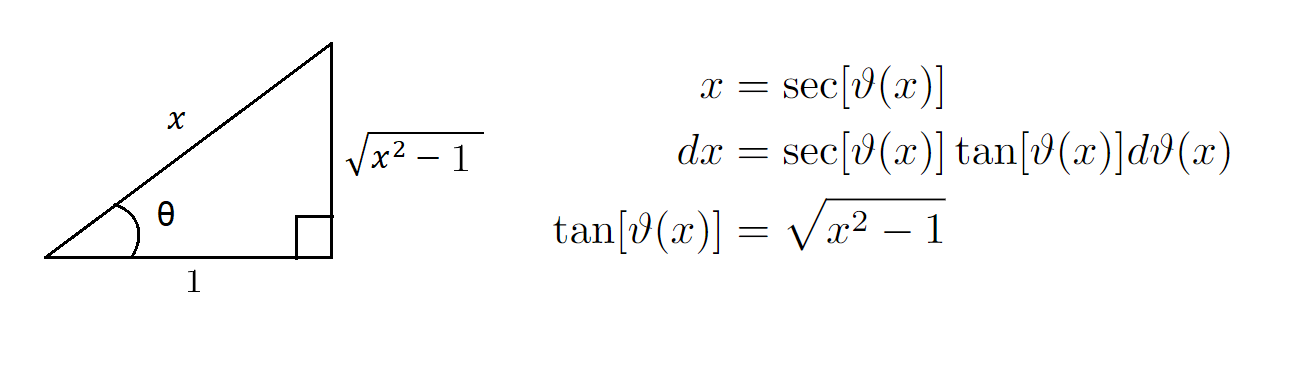
\includegraphics[width=0.6\linewidth]{trvarph.png}
    \label{fig:enter-label}
\end{figure} \\
%\begin{align*}
%    x &= \sec[\thetax] \\
%    dx &= \sec[\thetax]\tan[\thetax]d\thetax \\
%    \tan[\thetax] &= \sqrt{x^2-1}
%\end{align*} *\
\(
\ints x \, \sqrt{\frac{x-1}{x+1}} \, dx \cong \ints \sqrt{\frac{x^3-x^2}{x+1}} \, dx = \ints \frac{\sqrt{x^3-x^2}}{\sqrt{x+1}} \cdot \frac{\sqrt{x^3-x^2}}{\sqrt{x^3-x^2}} \, dx = \ints \frac{x^3-x^2}{\sqrt{x^4-x^2}} \, dx = \ints \frac{x^2-x}{\sqrt{x^2-1}} \, dx \\\\\\
= \ints \frac{x^2}{\sqrt{x^2-1}} \, dx - \ints \frac{x}{\sqrt{x^2-1}} \, dx = \ints \frac{\sec^2[\thetax]}{\tan[\thetax]}\sec[\thetax]\tan[\thetax]d\thetax - \ints \frac{\sec[\thetax]}{\tan[\thetax]}\sec[\thetax]\tan[\thetax]d\thetax \\\\\\
= \ints \sec^3[\thetax] d\thetax - \ints \sec^2[\thetax] d\thetax = \left[\ints \sec^3[\thetax] d\thetax\right] - \tan[\thetax] + c \\\\\\
\)
\textit{De acuerdo a la fórmula de reducción para la integral trigonométrica de la secante con exponente n de Leonhard Euler tenemos lo siguiente.}\\
\begin{align*}
    \mathbb{I}_n &= \ints \sec^n[\thetax] d\thetax = (n-1)^{-1}\sec^{n-2}[\thetax]\tan[\thetax] + \frac{n-2}{n-      1}\mathbb{I}_{n-2} \\
    \mathbb{I}_3 &= \ints \sec^3[\thetax] d\thetax = (3-1)^{-1}\sec^{3-2}[\thetax]\tan[\thetax] + \frac{3-2}{3-1}\mathbb{I}_{3-2} \\
    &= 2^{-1}\sec[\thetax]\tan[\thetax]+2^{-1}\mathbb{I}_1 \\
    &= 2^{-1}\cos^{-1}\frac{\sin[\thetax]}{\cos[\thetax]} + 2^{-1}\ints \sec[\thetax] d\thetax \\
    &= 2^{-1}\sec^2[\thetax]\sin[\thetax] + 2^{-1}\ints \sec[\thetax] d\thetax \\
    &= 2^{-1}\sec^2[\thetax]\sin[\thetax] + 2^{-1}\ln|\tan[\thetax]+\sec[\thetax]| \\
    &\ncong 2^{-1}\sec^2[\thetax]\sin[\thetax] + \ln(\sqrt{\tan[\thetax]+\sec[\thetax]})
\end{align*}\\
\textit{Esta última incongruencia es meramente señalatoria pues "introducir el exponente" nos recortaría el dominio $\mathbb{R^-}$, lo cual sería grave al intentar obtener la integral definida en intervalos del dominio negativos.}\\\\\\
\(
\implies \left[\ints \sec^3[\thetax] d\thetax\right] - \tan[\thetax] = 2^{-1}\sec^2[\thetax]\sin[\thetax] + 2^{-1}\ln|\tan[\thetax]+\sec[\thetax]| - \tan[\thetax] \\\\\\
= 2^{-1}x\sqrt{x^2-1} + 2^{-1}ln|\sqrt{x^2-1}+x| - \sqrt{x^2-1} + c
\)\\\\\\
\textit{Ahora bien, las propiedades algebráicas en ocasiones dictaminan congruencias que en realidad solo lo son parcialmente. Nótese que en el primer paso de la integral he "introducido" la x como $\sqrt{x^2}$; la razón de este señalización es que el dominio ha sido modificado de modo que: $\forall g(x) \in \mathbb{R^-}, \nexists y\in\mathbb{R^-} : y = (f\circ g)(x) = \sqrt{g(x)} $, véase esto en la gráfica (Figure I.) donde el trazo rojo corresponde a la función "antes de introducir la x", mientras que el azul al estar dentro del radical.}
\newpage
\textit{A lo que se pretende llegar con esto es que si se intenta graficar la integral mediante software (si es que siquiera logra resolver la integral) el resultado será incorrecto tal es el caso de geogebra en donde todo el rango de esta integral es positivo, cosa que analíticamente no es cierta; la línea continua negra es la primitiva que yo he deducido, quien respeta el signo de la función roja (original), recordemos que por definición la integral es la suma infinita de áreas en un sector y su signo está en función del eje ordenado, por lo cual nuestra primitiva está perfectamente definida.}
\begin{figure}[h]
    \centering
    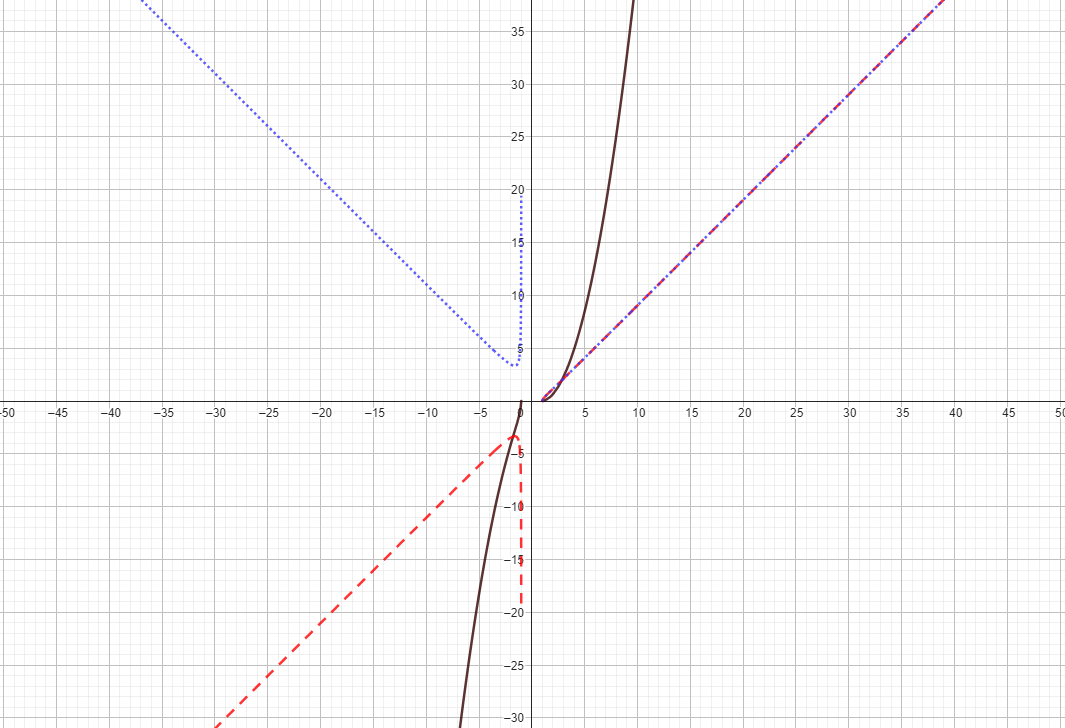
\includegraphics[width=0.6\linewidth]{fxgraph.png}
    \caption{Diferencia de rango por incongruencias algebráicas.}
    \label{fig:enter-label}
\end{figure} \\
$\therefore \ints x \, \sqrt{\frac{x-1}{x+1}} \, dx = 2^{-1}x\sqrt{x^2-1} + 2^{-1}ln|\sqrt{x^2-1}+x| - \sqrt{x^2-1} + c$
\\\\\\\\

% Problema XVII
\noindent XVII.  $\ints \frac{x^2+x+1}{x\sqrt{x^2-x+1}}$ = 
\begin{center}
\begin{tcolorbox}[title=Considérense en un futuro los siguientes cambios de variable, width=0.7\linewidth, top=0pt]
    \begin{align*}
    \phix = x - \frac{1}{2} \quad &\land \quad \mux = \frac{2\phix}{\sqrt{3}} = \frac{2x-1}{\sqrt{3}} \\
    d\phix = dx \quad &\land \quad d\mux \frac{2d\phix}{\sqrt{3}} \\
    \therefore \phix = \frac{\sqrt{3}\mux}{2} \quad &\land \quad d\phix = \frac{\sqrt{3}d\mux}{2} \\
    \end{align*}
\end{tcolorbox}
\end{center}
\(
\ints \frac{x^2+x+1}{x\sqrt{x^2-x+1}} = \ints \frac{(x+1)x+1}{x\sqrt{x^2-x+1}} \, dx = \ints \frac{xdx}{\sqrt{x^2-x+1}} + \ints \frac{dx}{\sqrt{x^2-x+1}} + \ints \frac{dx}{x\sqrt{x^2-x+1}}
\)\\\\
\textit{Resolvamos la primer integral de ellas.}\\\\
\(
\ints \frac{xdx}{\sqrt{x^2-x+1}} = \ints \frac{xdx}{\sqrt{(x-\frac{1}{2})^2+\frac{3}{4}}} = \ints \frac{\phix + \frac{1}{2}}{\sqrt{\phix^2+\frac{3}{4}}} \, d\phix = \ints \frac{(\phix+\frac{1}{2})d\phix}{\sqrt{\frac{3}{4}}\sqrt{\frac{\phix^2}{\frac{3}{4}}+1}} = \frac{2}{\sqrt{3}} \ints \frac{(\phix+\frac{1}{2})d\phix}{\sqrt{(\frac{2\phix}{\sqrt{3}})^2+1}} \\\\\\
= \frac{2}{\sqrt{3}} \ints \frac{\phix d\phix}{\sqrt{(\frac{2\phix}{\sqrt{3}})^2+1}} + \sqrt{3}^{-1} \ints \frac{d\phix}{\sqrt{(\frac{2\phix}{\sqrt{3}})^2+1}} = \frac{2}{\sqrt{3}} \ints \frac{\phix d\phix}{\sqrt{(\frac{2\phix}{\sqrt{3}})^2+1}} + \left[\frac{1}{\sqrt{3}}\right]\left[\frac{\sqrt{3}}{2}\right] \ints \frac{d\mux}{\sqrt{\mux^2+1}} \\\\\\
= \left[\frac{2}{\sqrt{3}} \ints \frac{\phix d\phix}{\sqrt{(\frac{2\phix}{\sqrt{3}})^2+1}}\right] + 2^{-1}\arcsinh[\mux] + c = \left[ \left[\frac{2}{\sqrt{3}}\right] \left[\frac{\sqrt{3}}{2}\right] \left[\frac{\sqrt{3}}{2}\right] \ints \frac{\mux d\mux}{\sqrt{\mux^2 +1}} \right] + 2^{-1}\arcsinh[\mux] + c
\)
\newpage
\begin{center}
\begin{tcolorbox}[title=Considérese el siguiente cambio de variable, width=0.7\linewidth, top=0pt]
    \[ \psix = \mux^2+1 = \frac{4\phix^2}{3}+1 \plic 2^{-1}d\psix = \mux \]
\end{tcolorbox}
\end{center}
\(
= \left[ \left[\frac{\sqrt{3}}{2}\right] \ints \frac{\mux d\mux}{\sqrt{\mux^2 +1}} \right] + 2^{-1}\arcsinh[\mux] + c = \left[ \left[\frac{\sqrt{3}}{4}\right] \ints \psix^{-\frac{1}{2}} d\psix \right] + 2^{-1}\arcsinh[\mux] + c \\\\\\
= \left[\frac{\sqrt{3}}{2}\right] \left[\frac{\sqrt{\psix}}{\frac{1}{2}}\right] + 2^{-1}\arcsinh[\mux] + c = 2^{-1}\sqrt{3\psix} + \frac{\arcsinh[\mux]}{2} + c = 2^{-1}\sqrt{4\phix^2 + 3} + \frac{\arcsinh[\frac{2x-1}{\sqrt{3}}]}{2} + c \\\\\\
= 2^{-1}\sqrt{4x^2-4x+4} + 2^{-1}\arcsinh\left[\frac{2x-1}{\sqrt{3}}\right] + c
\) \\\\
\textit{Recordemos que esto solo fue para calcular la primer integral... Operaremos con la segunda.}
\begin{center}
\begin{tcolorbox}[title=Hagamos un muy simple cambio de variable para hacer esto más visual, width=0.7\linewidth, top=0pt]
    \[ \xix = \frac{2\phix}{\sqrt{3}} \plic d\xix = \frac{2}{\sqrt{3}}d\phix \]
\end{tcolorbox}
\end{center}
\(
\ints \frac{dx}{\sqrt{x^2-x+1}} = \frac{2}{\sqrt{3}} \ints \frac{d\phix}{\sqrt{(\frac{2\phix}{\sqrt{3}})^2+1}} = \ints \frac{d\xix}{\sqrt{\xix^2+1}} = \arcsinh[\xix] + c = \arcsinh\left[\frac{2\phix}{\sqrt{3}}\right] + c \\\\\\
= \arcsinh\left[\frac{2(x - \frac{1}{2})}{\sqrt{3}}\right] + c = \arcsinh\left[\frac{2x-1}{\sqrt{3}}\right ] + c
\) \\\\
\textit{Finalmente resolveremos la última, la cual es con diferencia la más compleja de las 3; consideremos la siguiente sustitución trigonométrica.} \\
\begin{figure}[h]
    \centering
    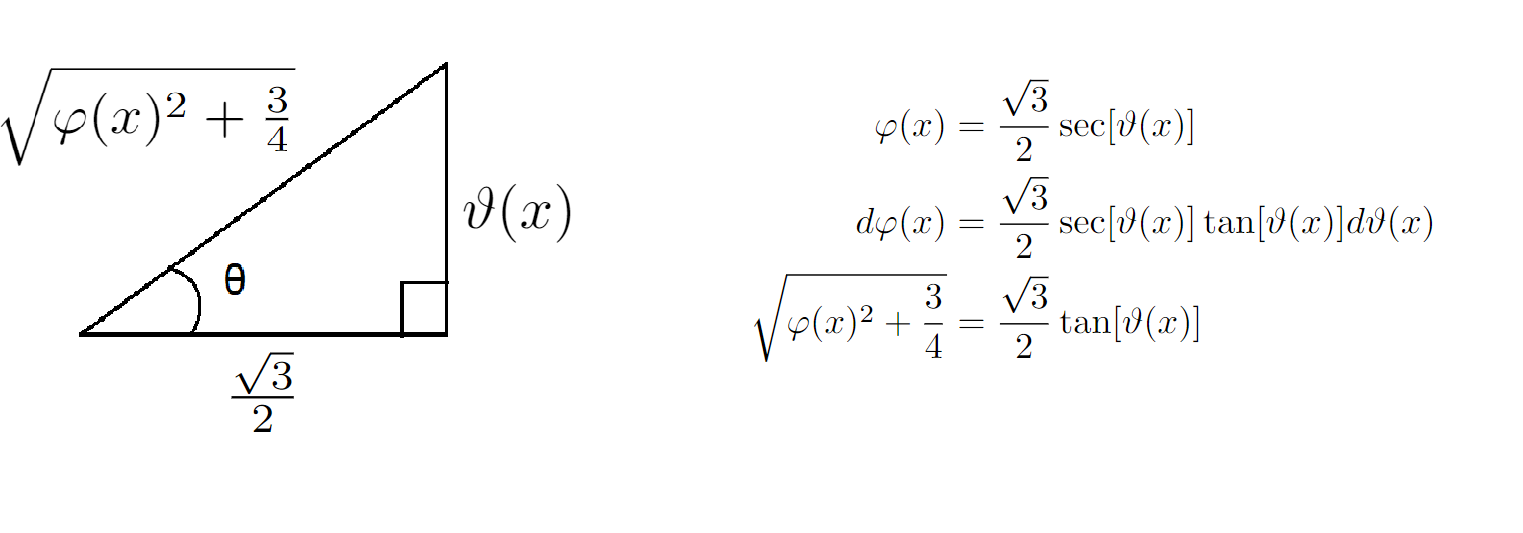
\includegraphics[width=0.6\linewidth]{trvarph2.png}
    \label{fig:enter-label}
\end{figure} \\
%\begin{align*}
%    \phix &= \frac{\sqrt{3}}{2} \sec[\thetax] \\
%    d\phix &= \frac{\sqrt{3}}{2} \sec[\thetax] \tan[\thetax] d\thetax \\
%    \sqrt{\phix^2+\frac{3}{4}} &= \frac{\sqrt{3}}{2} \tan[\thetax]
%\end{align*}

\(
\ints \frac{dx}{x\sqrt{x^2-x+1}} = \ints \frac{dx}{x\sqrt{(x-\frac{1}{2})^2+\frac{3}{4}}} = \ints \frac{d\phix}{(\phix+\frac{1}{2})\sqrt{\phix^2+\frac{3}{4}}} = \ints \frac{\frac{\sqrt{3}}{2}\sec[\thetax]\tan[\thetax]d\thetax}{(\frac{\sqrt{3}}{2}\sec[\thetax]+\frac{1}{2})\frac{\sqrt{3}}{2}\tan[\thetax]} \\\\\\
= \ints \frac{\sec\thetax d\thetax}{\frac{\sqrt{3}}{2}\sec[\thetax]+\frac{1}{2}}
\) \\\\
\textit{Nuevamente utilizamos sustitución trigonométrica.}
%\begin{align*}
%    \sin[\thetax] &= \frac{2\etax}{\etax^2+1} \\
%    \sec[\thetax] &= \frac{\etax^2+1}{1-\etax^2} \\
%    x &= \arctan[\frac{2\etax}{1-\etax^2}] \\
%    dx &= \frac{2d\etax}{\etax^2+1}
%\end{align*}
\begin{figure}[h]
    \centering
    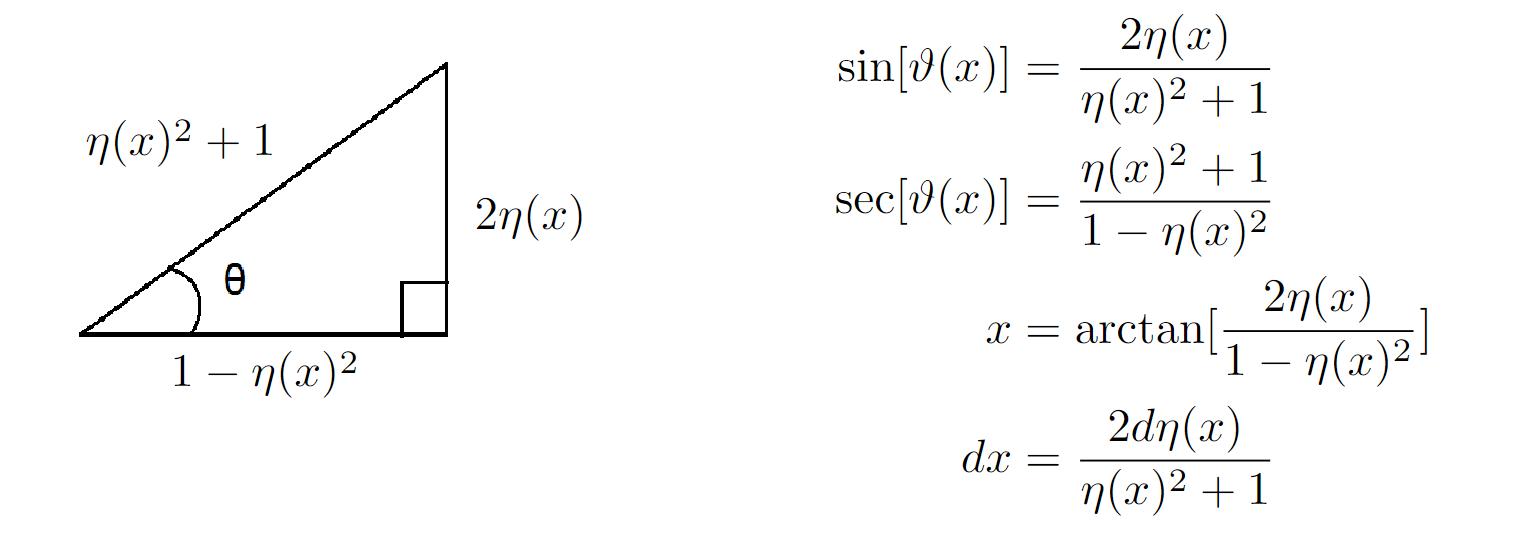
\includegraphics[width=0.6\linewidth]{trvarph3.png}
    \label{fig:enter-label}
\end{figure} \\
\(
\ints \frac{\sec\thetax d\thetax}{\frac{\sqrt{3}}{2}\sec[\thetax]+\frac{1}{2}} = \ints \frac{\left[\frac{\etax^2+1}{1-\etax^2}\right]\left[\frac{2d\etax}{\etax^2+1}\right]}{\frac{\sqrt{3}}{2}\left[\frac{\etax^2+1}{1-\etax^2}\right]+\frac{1}{2}} = \ints \frac{2d\etax}{(\frac{\sqrt{3}}{2}\left[\frac{\etax^2+1}{1-\etax^2}\right]+\frac{1}{2})(1-\etax^2)} = 2 \ints \frac{d\etax}{(\frac{\sqrt{3}}{2}\left[\frac{\etax^2+1}{1-\etax^2}\right]+\frac{1}{2})(1-\etax^2)}
\)
\newpage
\(
= 2 \ints \frac{d\etax}{-\frac{\etax^2}{2}+\frac{\sqrt{3}}{2-2\etax^2}-\frac{\sqrt{3}\etax^4}{2-2\etax^2}+\frac{1}{2}} = 2 \ints \frac{2d\etax(1-\etax^2)}{-\etax^2(1-\etax^2)+\sqrt{3}-\sqrt{3}\etax^4+(1-\etax^2)} \\\\\\
= 2\ints \frac{2d\etax(1-\etax^2)}{(1-\etax^2)(\sqrt{3}\etax^2-\etax^2+\sqrt{3}+1)} = 2 \ints \frac{2d\etax}{\sqrt{3}\etax^2-\etax^2+\sqrt{3}+1} = 4 \ints \frac{d\etax}{(1+\sqrt{3})(\frac{(\sqrt{3}-1)\etax^2}{1+\sqrt{3}}+1)} \\\\\\
= \frac{4}{1+\sqrt{3}} \ints \frac{d\etax}{\frac{(\sqrt{3}-1)\etax^2}{1+\sqrt{3}}+1}
\)
\begin{center}
\begin{tcolorbox}[title=Considérese el último cambio de variable, width=0.7\linewidth, top=0pt]
    \[ \upx = \sqrt{2-\sqrt{3}}\etax \plic d\upx = \sqrt{2-\sqrt{3}}d\etax\]
\end{tcolorbox}
\end{center}
\(
\frac{4}{1+\sqrt{3}} \ints \frac{d\etax}{\frac{(\sqrt{3}-1)\etax^2}{1+\sqrt{3}}+1} = \frac{4}{(1+\sqrt{3})\sqrt{2-\sqrt{3}}} \ints \frac{d\upx}{\upx^2+1} = \frac{4}{(1+\sqrt{3})\sqrt{2-\sqrt{3}}} \arctan[\upx] + c \\\\\\
= 2\sqrt{2} \arctan[\upx] + c = 2\sqrt{2} \arctan[\sqrt{2-\sqrt{3}}\etax] + c = 2\sqrt{2} \arctan\left[\sqrt{2-\sqrt{3}}(\tan\left[\frac{\thetax}{2}\right])\right] + c \\\\\\
= 2\sqrt{2} \arctan\left[\sqrt{2-\sqrt{3}}(\tan\left[\frac{(\arctan[\frac{2\phix}{\sqrt{3}}])}{2}\right])\right] + c = 2\sqrt{2} \arctan\left[\sqrt{2-\sqrt{3}}(\tan\left[\frac{(\arctan[\frac{2(x-\frac{1}{2})}{\sqrt{3}}])}{2}\right])\right] + c \\\\\\
= 2\sqrt{2} \arctan\left[\sqrt{2-\sqrt{3}}(\tan\left[\frac{(\arctan[\frac{2x-1)}{\sqrt{3}}])}{2}\right])\right] + c
\) \\\\
\textit{Como observación debido a la alta complejidad de esta última integral incluso geogebra falla al intentar calcularla pues en secciones positivas de la función original la integral adquiere valores negativos (de hecho en todo su rango lo hace); finalmente retomamos nuestras tres integrales iniciales.} \\\\
\(
\therefore \ints \frac{x^2+x+1}{x\sqrt{x^2-x+1}} = \ints \frac{xdx}{\sqrt{x^2-x+1}} + \ints \frac{dx}{\sqrt{x^2-x+1}} + \ints \frac{dx}{x\sqrt{x^2-x+1}} = \\\\\\
2^{-1}\sqrt{4x^2-4x+4} + 2^{-1}\arcsinh\left[\frac{2x-1}{\sqrt{3}}\right] + \arcsinh\left[\frac{2x-1}{\sqrt{3}}\right ] + 2\sqrt{2} \arctan\left[\sqrt{2-\sqrt{3}}(\tan\left[\frac{(\arctan[\frac{2x-1)}{\sqrt{3}}])}{2}\right])\right] + c
\)
\\\\\\\\

% Problema XVIII
\noindent XVIII.  $\ints \frac{dx}{\sqrt{x^3}(1+x^{\frac{3}{4}})^{\frac{1}{2}}}$ \\\\
\textit{De acuerdo a los 3 criterios de Integración por Binomio Diferencial establecidos en el teorema de Chebyshev, vemos que esta integral es una combinación infinita de funciones elementales por lo cual su resolución solo es posible mediante aproximaciones. Obsérvese que:} \\\\
\(
\ints \frac{dx}{\sqrt{x^3}(1+x^{\frac{3}{4}})^{\frac{1}{2}}} = \ints x^{-\frac{3}{2}}(1+x^{\frac{3}{4}})^{-\frac{1}{2}} \, dx = \ints x^{m}(1+x^{n})^{p} \, dx \\\\
p \notin \mathbb{Z} \\\\
\frac{m+1}{n} \notin \mathbb{Z} \\\\
\frac{m+1}{n}+p \notin \mathbb{Z} \\\\
\therefore \)
Esta integral de momento es imposible de resolver.
\\\\\\\\

% Problema XIX
\noindent XIX.  $\ints \sin^2[x]\cos^3[x] \, dx$
\begin{center}
\begin{tcolorbox}[title=Considérese en un futuro el siguiente cambio de variable, width=0.7\linewidth, top=0pt]
$\phix = \sin[x] \plic d\phix = \cos[x]dx$
\end{tcolorbox}
\end{center}
\(
\ints \sin^2[x]\cos^3[x] \, dx = \ints \cos^2[x]\sin^2[x]\cos[x] \, dx = \ints (1 - \sin^2[x])\sin^2[x]\cos[x] \, dx = \ints (1 - \phix^2)\phix^2 d\phix \\\\\\
= \ints \phix^2 d\phix - \ints \phix^4 d\phix = 3^{-1}\phix^3 - 5^{-1}\phix^5 + c = 3^{-1}\sin[x]^3 - 5^{-1}\sin[x]^5 + c 
\)
\\\\\\\\

% Problema XX
\noindent XX.  $\ints \cos^6[3x] \, dx$ \\\\
\textit{De acuerdo a la fórmula de reducción para la integral trigonométrica del coseno con exponente n de Leonhard Euler tenemos lo siguiente.}\\
\(
\mathbb{I}_n = \ints \cos^n[\phix] d\phix = n^{-1}cos^{n-1}[\phix]\sin[\phix] + \frac{n-1}{n}\mathbb{I}_{n-2} \\\\\\
\implies \mathbb{I}_6 = 3^{-1}[6^{-1}\cos^5[\phix]\sin[\phix] + \frac{5}{6}(4^{-1}\cos^3[\phix]\sin[\phix] + \frac{3}{8}(\phix + 2^{-1}\sin[2\phix]))] + c \\\\\\
\therefore \ints \cos^6[3x] \, dx = 3^{-1}[6^{-1}\cos^5[3x]\sin[3x] + \frac{5}{6}(4^{-1}\cos^3[3x]\sin[3x] + \frac{3}{8}(3x + 2^{-1}\sin[6x]))] + c 
\)
\\\\\\\\

% Problema XXI
\noindent XXI.  $\ints \sin[x] \sinh[x] \, dx$
\begin{center}
\begin{tcolorbox}[title=Considérense las siguientes variables para la integración por partes., width=0.7\linewidth, top=0pt]
    \begin{align*}
        u = \sin[x] \quad &\land \quad v = \cosh[x] \\
        du = \cos[x] \quad &\land \quad dv = \sinh[x]
    \end{align*}
\end{tcolorbox}
\end{center}
\(
\ints \sin[x] \sinh[x] \, dx = \sin[x] \cosh[x] - \ints \cos[x] \cosh[x] dx
\)
\begin{center}
\begin{tcolorbox}[title=Considérense estas nuevas variables para la integración por partes., width=0.7\linewidth, top=0pt]
    \begin{align*}
        \textbf{u} = \cos[x] \quad &\land \quad \textbf{v} = \sinh[x] \\
        \textbf{du} = -\sin[x] \quad &\land \quad \textbf{dv} = \cosh[x]
    \end{align*}
\end{tcolorbox}
\end{center}
\(
\sin[x] \cosh[x] - \ints \cos[x] \cosh[x]dx = \sin[x]\cosh[x] - \cos[x] \sinh[x] - \ints \sin[x] \sinh[x] dx
\) \\\\
\textit{Retomamos...} \\
\begin{align*}
    \ints \sin[x] \sinh[x] \, dx &= \sin[x]\cosh[x] - \cos[x]\sinh[x] - \ints \sin[x]\sinh[x] dx \\
    2\ints \sin[x] \sinh[x] \, dx &= \sin[x]\cosh[x] - \cos[x]\sinh[x] \\
    \therefore \ints \sin[x] \sinh[x] \, dx &= 2^{-1}(\sin[x]\cosh[x] - \cos[x]\sinh[x])
\end{align*}
\\\\\\\\

% Problema XXII
\noindent XXII.  Si $\mathbb{I}_n = \ints x^n e^{-x} dx $ calcular $\mathbb{I}_{10} = \ints x^{10} e^{-x} dx $ \\\\
\textit{Se utilizará el método de integración por tabulación. Es particularmente eficiente en integrales de este tipo y consiste en calcular la integral indefinida mediante integración por partes repetidamente, donde una de las funciones se deriva y la otra se integra en cada paso. Luego, se tabulan los resultados obtenidos para cada iteración y se aplican las condiciones iniciales o finales, según sea necesario, para encontrar la solución final; la siguiente tabla es la iteración repetida de la integración por partes, bastará con multiplicar en diagonal y sumar cada uno de estos productos para obtener la integral final.}
\begin{center}
\begin{array}{|c|c|}
\hline
D_x & D_e \\
\hline
x^{10} & e^{-x} \\
10x^9 & -e^{-x} \\
90x^8 & e^{-x} \\
720x^7 & -e^{-x} \\
5040x^6 & e^{-x} \\
30240x^5 & -e^{-x} \\
151200x^4 & e^{-x} \\
604800x^3 & -e^{-x} \\
1814400x^2 & e^{-x} \\
10!x & -e^{-x} \\
10! & e^{-x} \\
\hline
\end{array}
\end{center}
\(
\mathbb{I}_{10} = \ints x^{10} e^{-x} dx \\\\\\
= e^{-x}(-x^{10} - 10x^9 - 90x^8 - 720x^7 - 5040x^6 - 30240x^5 - 151200x^4 - 604800x^3 - 1814400x^2 - 10!x - 10!) + c
\) \\\\\\\\\\\\\\

% Casi muero haciendo esto :C

\end{document}